The \gls{qmla} framework lends itself easily to the family of optimsation techniques called \emph{evolutionary algorithms}, 
    where individuals, sampled from a population of candidates, are considered, in generations, as solutions to the given problem,
    and iterative generations aim to efficiently search the available population, 
    by mimicing biological evolutionary mechanisms \cite{back1996evolutionary}. 
In particular, we develop a \gls{es} which incorporates an \gls{ga} in the generation of models;
    \glspl{ga} are a subset of evolutionary algorithms where candidate solutions are expressed as 
    strings of numbers representing some configuration of the system of interest \cite{holland1992adaptation}.
Here we will first introduce the concept of a \gls{ga}, before describing the adaptations which allow us to 
    build a \gls{ges}. 

\section{Genetic algorithm definition}
\glspl{ga} work by assuming a given problem can be optimised, if not solved, by a single candidate 
    among a fixed, closed space of candidates, called the population, $\population$. 
A number of candidates are sampled at random from $\population$ into a single \emph{generation}, 
    and evaluated through some \gls{of}, which assesses the fitness of the candidates at solving the problem of interest. 
Candidates from the generation are then mixed together to produce the next generation's candidates: 
    this \emph{crossover} process aims to combine only relatively strong candidates, such that the average 
    candidates' fitness improve at each successive generation, 
    mimicing the biological mechanism whereby the genetic makeup of offspring is an even mixture of both parents. 
The selection of strong candidates as parents for future generations is therefore imperative; 
    in general parents are chosen according to their fitness as determined by the \gls{of}. 
Buidling on this biological motivation, much of the power of \glspl{ga} comes from the concept of \emph{mutation}: 
    while offspring retain most of the genetic expressions of their parents, some elements are mutated at random.
Mutation is crucial in avoiding local optima of the \gls{of} landscape
    by maintaining diversity in the examined subspace of the population.
\par 

Pseudocode for a generic \gls{ga} is given in \cref{alg:ga},
    but we can also informally define the procedure as follows. 
Given access to the population, $\population$, 

\begin{easylist}[enumerate]
    \ListProperties(Numbers2=l, Numbers3=r)
    & Sample $N_m$ candidates from the population at random
    && call this group of candidates the first generation, $\mu$. 
    & \label{ga:loop} Evaluate each candidate $\gamma_j \in \mu$. 
    && each $\gamma_j$ is assigned a fitness, $g_j$
    && the fitness is computed through an objective function acting on the candidate, $g(\gamma_j)$. 
    & Map the fitnesses of each candidate, $\{g_j\}$, to selection probabilities for each model, $\{s_j\}$
    && e.g. by normalising the fitnesses, or by removing some poorly-performing candidates and then normalising. 
    & Generate the next generation of candidates, $\mu^{\prime}$
    && $\mu = \{ \}$
    && \label{ga:select} Select pairs of parents, $p_1, p_2$, from $\mu$
    &&& Each candidate's probability of being chosen is given by their $s_j$
    && Cross over $p_1,p_2$ to produce children candidates, $c_1,c_2$. 
    &&& mutate $c_1, c_2$ according to some random probabilistic process
    &&& keep $c_i$ only if it is not already in $\mu^{\prime}$, to ensure $N_m$ unique models are tested at each generation.
    && until $| \mu^{\prime}| = N_m$, iterate to step (\ref{ga:select}.
    & Until the $N_g^{th}$ generation is reached, iterate to step \ref{ga:loop}.
    & The strongest candidate on the final generation is deemed the solution to the posed problem. 
\end{easylist}


\begin{algorithm}
    \caption{Genetic algorithm}
    \label{alg:ga}
    \DontPrintSemicolon
    \KwIn{ $\population$ \tcp*[1]{Population of candidate models}}
    \KwIn{ $g()$ \tcp*[1]{objective funtion}}
    \KwIn{ $\ttt{map\_g\_to\_s}()$ \tcp*[1]{function to map fitness to selection probability}}
    \KwIn{ $\ttt{select\_parents}()$ \tcp*[1]{function to select parents among generation}}
    \KwIn{ $\ttt{crossover}()$ \tcp*[1]{function to cross over two parents to produce offspring}}
    \KwIn{ $N_g$ \tcp*[1]{number of generations}}
    \KwIn{ $N_m$ \tcp*[1]{number of candidates per generation}}\;

    \KwOut{$\gamma^{\prime}$ \tcp*[1]{strongest candidate}}\;
    
    $\mu \gets \ttt{sample} \left( \population, N_m\right)$\; 

    \For{$i \in 1, ..., N_g$}{
        \For{$\gamma_j \in \mu$ }{
            $g_j \gets g(\gamma_j) $ \tcp*[1]{assess fitness of candidate}
        }

        $\{ s_j \}  \gets \ttt{ map\_g\_to\_s}(\{g_j \})$ \tcp*[1]{map fitnesses to normalised selection probability}
        $\mu_c = \argmax\limits_{s_j} \{ \gamma_j \}$ \tcp*[1]{record champion of this generation}\;

        $\mu \gets \{ \}$ \tcp*[1]{empty set for next generation}

        \While{$| \mu | < N_m$}{
            $p_1, p_2 \gets \ttt{select\_parents}(\{s_j\})$ \tcp*[1]{choose parents based on candidates' $s_j$}
            $c_1, c_2 \gets \ttt{crossover}(p_1,p_2)$ \tcp*[1]{generate offspring candidates based on parents}

            \For{$c \in \{c_1, c_2\}$ }{
                \If{$c \notin \mu$}{
                    $\mu \gets \mu \cup \{ c\}$ \tcp*[1]{keep if child is new} 
                }
            }
        }
    }

    $\gamma^{\prime} \gets \argmax\limits_{s_j}\{ \gamma_j \in \mu \}$ \tcp*[1]{strongest candidate on final generation}\;

    return $\gamma^{\prime}$

\end{algorithm}


\par 

Candidates are manifested as \emph{\glspl{chromosome}}, i.e. strings of fixed length, 
    whose entries, called  \emph{\glspl{gene}}, each represent some element of the system.
In general, \glspl{gene} can have continuous values, although usually, and for all purposes in this thesis, 
    genes are binary, capturing simply whether or not the \gls{gene}'s corresponding feature is present 
    in the \gls{chromosome}. 

\subsection{Example: knapsack problem}
One commonly referenced combinatorial optimisation problem is the \emph{knacksack problem}: 
    given a set of objects, where each object has a defined mass and also a defined value, 
    determine the set of objects to pack in a knapsack which can support a limited weight, 
    such that the value of the packed objects is maximised. 
Say there are $n$ objects, 
    we can write the vector containing the values of those objects as $\vec{v}$, 
    and the vector of their weights as $\vec{w}$. 
We can then represent configurations of object sets as candidate vectors $\vec{\gamma}_j$, 
    whose genes are binary, and simply indicate whether or not the associated object is included in the set. 
For example, with $n=6$,
\begin{equation}
    {\gamma}_j = $\ttt{100001} \Longrightarrow $\vec{\gamma}_j = \irow{1 & 0 & 0 & 0 & 0 & 1},
\end{equation} 
indicates a set of objects consisting only of those indexed first and last, with none of the intermediate objects included. 

\par
The fitness of any candidate is then given by the total value of that configuration of objects, $v_j = \vec{v} \cdot \vec{\gamma}_j$, 
    but candidates are only admitted\footnotemark \ if the weight of the corresponding set of objects 
    is less than the capacity of the knapsack, i.e. $\vec{w}_j \cdot \vec{\gamma}_j \leq w_{max}$. 
\footnotetext{
    Note there are alternative strategies to dealing with candidates who violate the weight condition, 
    such as to impose a penalty within the \gls{of}, but for our purposes let us assume we simply disregard violators. 
}
\par 

For example where each individual object has value $<50$ and weight $<25$ and $w_{max} = 50$, 
recalling $\gamma_j = \ttt{100001}$, say, 
\begin{subequations}
    \begin{equation}
        \vec{ v } = \irow{ 48 & 15 & 26 & 19 & 39 & 15 } \Longrightarrow v_j = \vec{\gamma}_j \cdot \vec{v} = 48 + 15 = 63;
    \end{equation}
    \begin{equation}
        \vec{ w } = \irow{ 21 & 7 & 2 & 17 & 10 & 20 } \Longrightarrow w_j = \vec{\gamma}_j \cdot \vec{w} = 21 + 20 = 41.
    \end{equation}
\end{subequations}
We can hence assess the fitness of $\gamma_j$ as $63$ and deem it a valid candidate since it does not exceed the weight threshold.
We can likewise compute the total weight and value of a series of randomly generated candidates, 
    and deem them valid or not. 

\begin{table}[H]
    \begin{center}
        \begin{tabular}{lrrl}
\hline
{} &                                    Value &                                   Weight &                                    Valid \\
Candidate                                &                                          &                                          &                                          \\
\midrule
110000                                   &                                       63 &                                       28 &                                      Yes \\
000011                                   &                                       54 &                                       30 &                                      Yes \\
011101                                   &                                       75 &                                       46 &                                      Yes \\
101010                                   &                                      113 &                                       33 &                                      Yes \\
000101                                   &                                       34 &                                       37 &                                      Yes \\
010111                                   &                                       88 &                                       54 &                                       No \\
011011                                   &                                       95 &                                       39 &                                      Yes \\
110011                                   &                                      117 &                                       58 &                                       No \\
000000                                   &                                        0 &                                        0 &                                      Yes \\
110001                                   &                                       78 &                                       48 &                                      Yes \\
100010                                   &                                       87 &                                       31 &                                      Yes \\
011110                                   &                                       99 &                                       36 &                                      Yes \\
\hline
\end{tabular}

        \caption[Candidate solutions to knapsack problem]{
            Candidate solutions to the knapsack problem. 
        }
        \label{table:knapsack_candidates}
    \end{center}
\end{table}

The strongest (valid) candidates from \cref{table:knapsack_candidates} are \ttt{101010}, \ttt{011110}. 
By spawning from these candidates through a one-point crossover at the midpoint, 
    we get $\gamma_{c_1} = \ttt{101110}, \gamma_{c_2} = \ttt{011010}$, 
    from which we can see $v_{c_1} = 132, w_{c_1} = 50$, i.e. by combining two strong candidates we produce 
    the strongest-yet-seen valid candidate. \par 

By repeating this procedure, it is expected to uncover candidates which optimise $v_j$ while maintining $w_j \leq w_{max}$, 
    or at least to produce near-optimal solutions, using far less time/resources than brute-force evaluation of all candidates, 
    which is usually sufficient. 
For instance, with $n=100$ objects to consider, there are $2^{100} \approx 10^{30}$ candidates to consider; 
    the most powerful supercomputers in the world currently claim on the order of Exa-FLOPs, 
    i.e. $10^{18}$ operations per second, of which say $\sim1000$ operations are required to test each candidate, 
    meaning $10^{15}$ candidates can be checked per second in a generous example. 
This would still require $10^{12}$ seconds to solve absolutely, 
    so it is reasonable in cases like this to accept 
    \emph{approximately optimal} solutions\footnote{
        Simply put: in machine learning, \emph{good enough} is good enough.
        We will adopt this philosophy for the remainder of this thesis and life. 
    }. 


\subsection{Selection mechanism}
A key subroutine of every \gls{ga} is the mechanism through which it nominates candidates fromm generation $g$ 
as parents to offsping candidates in $g+1$ \cite{luke11}. 
All mechanisms have in common that they act on a set of candidates from the previous generation, 
    where each candidate, $\gamma_j$, has been evaluated and has fitness value, $g_j$. 
Among the viable schemes for selecting individual parents from the set of candidates, $\mu$  are
\begin{easylist}[itemize]
    & Rank selection: candidates are selected with probabilty proportional to their ranking relative to 
        the fitness of contemporary candidates in the same generation. 
    & Tournament selection: a subset of $k$ candidates are chosen at random from $\mu$, 
        of which the candidate with the highest fitness is taken as the parent. 
    & Stochastic universal sampling: candidates are sampled proportional to their fitness, 
        but the sampling algorithm is biased to ensure high-fitness candidates are chosen at least once 
        within the generation. 
\end{easylist}

We will only detail the mechanism used later within \gls{qmla}, 
    the common fitness proportional selection, known as \emph{roulette selection} \cite{luke11}. 
This is a straightforward strategy where we directly map candidates' fitness, $g_i$ to a selection probability, $s_i$,
    simply by normalising $\{g_i\}$, 
    allowing us to visualise a roulette wheel of uneven wedges, eachh of which correspond to a candidate. 
Then we need only conceptually spin the roulette wheel to select the first parent, $\gamma_{p_1}$. 
We then remove $\gamma_{p_1}$ from the set of potential parents, renormalise the remaining $\{s_i\}$, 
    and spin the wheel again to choose the second parent, $\gamma_{p_2}$. 
\par 
Practically, we repeat the process outlined until the next generation is filled, 
    usually we have $|\mu| = N_m$, and desire that every generation should contain the same 
    $N_m$ candidates, so we repeat the roulette selection $\nicefrac{N_m}{2}$ times per generation, 
    since every pair of parents yield two offspring.
It is important that meaningful differences in fitness are reflected by the selection probability, 
    which is difficult to ensure for large $N_m$, e.g. with ten models, the strongest candidate is only 
    a marginally more probable parent than the worst -- this effect is amplified for larger $N_m$. 
We therefore wish to reduce the set of potential parents to ensure high quality offspring:
    we truncate $\mu$ and retain only the highest-fitness $\frac{N_m}{2}$ models as selectable parents. 
The roulette selection is shown in \cref{fig:knapsack_roulette}\textbf{a-c}. 

\begin{figure}
    \begin{center}
        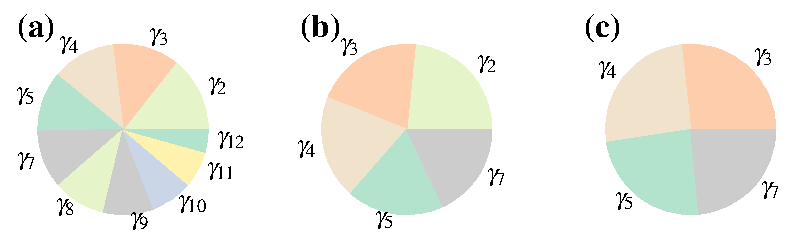
\includegraphics{theoretical_study/figures/knapsack_roulette.pdf}
    \end{center}
    \caption[Roulette wheels for selection]{
        Roulette wheels showing selection probability $s_i$ for corresponding candidates $\gamma_i$. 
        Colours here only distinguish candidates, they do not encode any information. 
        \textbf{a}, All valid candidates are assigned selection probability based on their value in \ref{table:knapsack_candidates}. 
        \textbf{b}, The set of potential parents is truncated to include only the strongest five candidates. 
        \textbf{c}, After one parent ($\gamma_2$) has been chosen, it is removed from the roulette wheel and the remaining
         candidates' probabilities are renormalised for the selection of the second parent. 
    }
    \label{fig:knapsack_roulette}
\end{figure}

\subsection{Offspring production}
crossover and mutation mechanisms

\subsection{Candidate evaluation}


\section{Adaptation to QMLA framework}


% TODO uncomment the algorithm below - excluded for readibility of other sections
% \begin{algorithm}
%     \caption{ES subroutine: \ttt{generate\_models} (example: genetic algorithm)}
%     \label{alg:generate_models}
%     \DontPrintSemicolon
%     \KwIn{ $\nu$ \tcp*[1]{information about models considered to date}}\;
%     \KwIn{ $g(\hi)$ \tcp*[1]{objective function}}\;

%     \KwOut{$\mathbb{H}$ \tcp*[1]{set of models}}\;
    
%     $ N_m = \left| \nu \right| $ \tcp*[1]{number of models}

%     \For{$\hi \in \nu$}{
%        $g_i \gets g(\hi)$ \tcp*[1]{model fitness via objective function}
%     }
%     $r \gets $ \ttt{rank($\{ g_i \}$)} \tcp*[1]{rank models by their fitness}
%     $\mathbb{H}_t \gets $ \ttt{truncate($r, \frac{N_m}{2}$)} \tcp*[1]{truncate models by rank: only keep $\frac{N_m}{2}$}
%     $ s \gets $ \ttt{normalise($\{g_i\}$)} $\forall \hi \in \mathbb{H}_t$ \tcp*[1]{normalise remaining models' fitness}

%     $\mathbb{H} = \{\}$ \tcp*[1]{new batch of chromosomes/models}

%     \While{ $\left| \mathbb{H} \right| < N_m$ }{
%         $p_1, p_2 = $ \ttt{roulette($s$)} \tcp*[1]{use $s$ to select two parents via roulette selection}
    
%         $c_1, c_2$ = \ttt{crossover($p_1, p_2$)} \tcp*[1]{produce offspring models}

%         $c_1, c_2$ = \ttt{mutate($c_1, c_2$)} \tcp*[1]{probabilistically mutate}

%         $\mathbb{H} \gets \mathbb{H} \cup \{ c_1, c_2 \} $ \tcp*[1]{add new models to batch}

%     }

%     % \ttt{roulette($s$)}

%     return $\mathbb{H}$ 

% \end{algorithm}



\section{Objective functions}

\section{Application}